\documentclass[11pt, letterpaper]{article}
\setlength{\parindent}{0in}
\setlength{\textheight}{8.7in}
\setlength{\textwidth}{6.8in}
\setlength{\oddsidemargin}{-0.3in}
\setlength{\evensidemargin}{0.0in}
\addtolength{\topmargin}{-1in}
\setlength{\parskip}{0.1in}

\usepackage{amsmath, amsfonts, color}
\usepackage{amssymb}
\usepackage{bm}
\usepackage{booktabs}
\usepackage{enumerate}
\usepackage{graphicx}
\usepackage{hyperref}
\newcommand*{\justifyheading}{\raggedleft}


\renewcommand{\baselinestretch}{1.0}

\newcommand{\bx}{{\bm x}}
\newcommand{\bX}{{\bm X}}
\newcommand{\by}{{\bm y}}
\newcommand{\bY}{{\bm Y}}
\newcommand{\bW}{{\bm W}}
\newcommand{\bG}{{\bm G}}
\newcommand{\bR}{{\bm R}}
\newcommand{\bZ}{{\bm Z}}
\newcommand{\bV}{{\bm V}}
\newcommand{\bL}{{\bm L}}
\newcommand{\bz}{{\bm z}}
\newcommand{\be}{{\bm e}}
\newcommand{\bgamma}{{\bm \gamma}}
\newcommand{\bbeta}{{\bm \beta}}
\newcommand{\balpha}{{\bm \alpha}}
\newcommand{\bSigma}{{\bm \Sigma}}
\newcommand{\bmu}{{\bm \mu}}
\newcommand{\btheta}{{\bm \theta}}
\newcommand{\bepsilon}{{\bm \epsilon}}
\newcommand{\bone}{{\bm 1}}
\newcommand{\bzero}{{\bm 0}}
\newcommand{\bC}{{\bm C}}
\newcommand{\bI}{{\bm I}}
\newcommand{\bA}{{\bm A}}
\newcommand{\bB}{{\bm B}}
\newcommand{\bQ}{{\bm Q}}
\newcommand{\bS}{{\bm S}}
\newcommand{\bD}{{\bm D}}
\newcommand{\cQ}{\mathcal{Q}}
\newcommand{\cU}{\mathcal{U}}
\newcommand{\cI}{\mathcal{I}}
\newcommand{\cL}{\mathcal{L}}

\newcommand{\beas}{\begin{eqnarray*}}
\newcommand{\eeas}{\end{eqnarray*}}

\newenvironment{equationarrayright}{
                          \begin{eqnarray*}
                          \begin{array}{rcll}
                         }{
                          \end{array}
                          \end{eqnarray*}
                         }
\newcommand{\bear}{\begin{equationarrayright}}
\newcommand{\eear}{\end{equationarrayright}}

\renewcommand\arraystretch{1.3}

\DeclareMathOperator*{\argmin}{arg\,min}

\title{STAT/BIOST 571: Homework 1}
\date{\today}
\author{Philip Pham}

\begin{document}

\maketitle

\section*{Problem 1: Non-parametric linear regression (5 points)}
{In the context of random $\bX$ linear regression, consider $n$ independent observations $(x_i, Y_i)$ generated as follows.  
First, the indepenent variable $x_i$ is selected according to 
\[
x_i = \left\{ \begin{array}{cl} 0 & \textrm{w.p. 1/3} \\  
                                          1 & \textrm{w.p. 1/3} \\ 
                                          3 & \textrm{w.p. 1/3} \end{array} \right. ,
\]
then the systematic component of $Y_i$ is set to
\[
\mu_i = \left\{ \begin{array}{cl} 0.6 & \textrm{if } x_i = 0 \\  
                                           3.6& \textrm{if } x_i=1 \\ 
                                          6.8 &\textrm{if } x_i=3 \end{array} \right. ,
\]
and finally $Y_i \sim N(\mu_i , \sigma^2)$ with $\sigma^2=1$.  
\begin{enumerate}[(a)]
{\item Simulate a single realization from the data-generating mechanism described above (with $n=20$)
and present the data in a scatterplot, with the $Y_i$ on the vertical axis and the $x_i$ on the horizontal axis.  Fit a simple linear regression model of the form
\[
Y_i = \beta_0 + x_i \beta_1 + \epsilon_i
\]
by ordinary least squares and overlay the fitted regression line on your scatterplot.  Comment on the approporiateness of fitting a linear model to these data.}

\begin{description}
\item[Solution:] See Figure \ref{fig:p1_ols}. 
  
  \begin{figure}
    \centering
    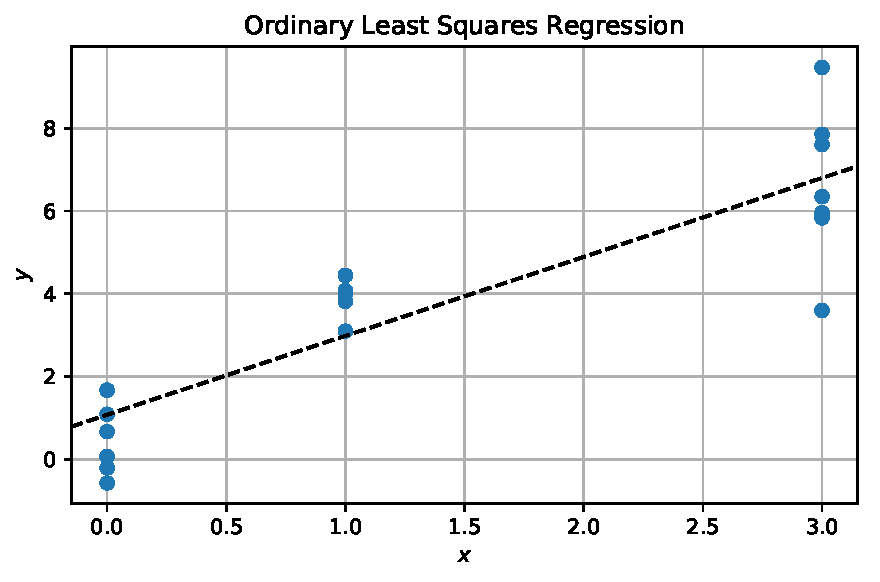
\includegraphics{p1_ols.pdf}
    \caption{Ordinary least squares for data according to the model in Problem 1.}
    \label{fig:p1_ols}
  \end{figure}

  The line isn't a very good fit. It overestimates when $x = 0$ and
  underestimates when $x = 1$. This isn't surprising since the linear model is
  incorrect.
  
\end{description}
{\item Let $\hat{\beta}_1$ be the estimated slope parameter from fitting the model above, and define $\beta_1$ to be the quantity for which $\hat{\beta}_1$ is consistent, in the limit as $n \rightarrow \infty$.  Using the result on Slide 1.18 of the course lecture notes, calculate $\beta_1$ exactly.}

\begin{description}
\item[Solution:] $\beta_0 = 1$ and $\boxed{\beta_1 = 2.}$
  
  Let $\mathbb{P}$ be the probability measure over $x$ and $y$. Let
  $\phi\left(x \mid \mu, \sigma^2\right)$ be the density of the normal
  distribution with mean $\mu$ and variance $\sigma^2$. Consider the integral,
  \begin{align*}
    L\left(\gamma\right)
    &= \int \left(y - \left(\gamma_0 + \gamma_1x\right)\right)^2\,\operatorname{d}\mathbb{P}\left(x, y\right) \\
    &= \frac{1}{3}\int_{-\infty}^\infty\left(y - \gamma_0\right)^2\phi\left(y\mid 0.6, 1\right)\,\operatorname{d}y + \\
    &~~~~\frac{1}{3}\int_{-\infty}^\infty\left(y - \gamma_0 - \gamma_1\right)^2\phi\left(y\mid 3.6, 1\right)\,\operatorname{d}y + \\
    &~~~~\frac{1}{3}\int_{-\infty}^\infty\left(y - \gamma_0 - 3\gamma_1\right)^2\phi\left(y\mid 6.8, 1\right)\,\operatorname{d}y \\
    &= \frac{1}{3}\left(
      62.56 - 22\gamma_0 - 48\gamma_1 + 3\gamma_0^2 + 10\gamma_1^2 + 8\gamma_0\gamma_1
      \right).      
  \end{align*}
  If we let $\beta = \argmin_\gamma L\left(\gamma\right)$. Taking the
  derviative, we setting
  $\frac{\partial L }{\partial \gamma}\left(\beta\right) = 0$ to obtain
  $\beta_0 = 1$ and $\beta_1 = 2$.
\end{description}

{\item Download White's seminal paper from 1980 on sandwich estimation from the course website .  Read (at least) the first few pages and explain how the value of $\beta_1$ you derived in part (b) also follows
  from Lemma 1 of the paper.}

\begin{description}
\item[Solution:] In fitting the model, we are assuming that the linear model is
  correct and Assumption 1 of the paper holds.

  Assumption 2 is satisfied so since $\mathbb{E}\left[\epsilon_i^2\right] = 1$
  for all $i$ and the expected covariance matrix =
  $\bar{M}_n = n^{-1}\sum_{i=1}^n\mathbb{E}\left[X_i^2\right]$ is just a matrix
  $1 \times 1$ with a single positive entry, so it is certainly nonsingular is
  with a positive determinant.

  Thus, Lemma 1 tells us that $\hat{\beta} \xrightarrow {\mathrm{a.s.}} \beta$,
  where $\hat{\beta} = \left(X^\intercal X\right)^{-1} X^\intercal Y$.

  Since $\hat{\beta}$ is also the maximum likelihood estimate which minimizes
  mean squared error, it converges almost surely to the value of $\beta$ that
  minimizes expected mean squared error.
\end{description}

{\item For finite $n$, we cannot discuss properties of the expectation of $\hat{\beta}_1$, at least not in the conventional sense.  Explain why not.}

\begin{description}
\item[Solution:] Note that
  $\hat{\beta} = \left(X^\intercal X\right)^{-1} X^\intercal Y$.  

  If the linear model were correct, that is, $Y = X\beta + \epsilon$, taking the
  expection would give
  \begin{equation}
    \mathbb{E}\left[\hat{\beta}\right]
    = \beta + \mathbb{E}\left[
      \left( X^\intercal X \right)^{-1} X^\intercal \epsilon
    \right] = \beta.
  \end{equation}

  However, This calculation is incorrect when $Y$ depends on $X$ in a non-linear
  way as with these data.
\end{description}

\end{enumerate}
For the remainder of this problem, condition on realizations of the data for which there exist $i$ and $i^\prime$ such that $x_i \neq x_{i^\prime}$.
\begin{enumerate}[(a)] \addtocounter{enumi}{4}
{\item Conduct a simulation study to assess the bias of $\hat{\beta}_1$ for estimating $\beta_1$.  Plot the estimated bias as a function of $n$ (for $n=2,4,6,\ldots,28,30,35,\ldots,95,100$), and overlay the standard error of $\hat{\beta}_1$ as a function of $n$.  Note that for this problem you should estimate the standard error of $\hat{\beta}_1$ based on the 
  standard deviation of $\hat{\beta}_1$ across simulated realizations of the data, not using any further exact or asymptotic calculations.}

\begin{description}
\item[Solution:] See Table \ref{tab:p1_simulation_results} for the slope
  estimates $\hat{\beta}_1$ and standard error estimates $\hat{\sigma}$ for
  different values of $n$.

  \begin{table}
    \centering
    \begin{tabular}{rrrr}
\toprule
 $n$ &  $\hat{\beta}_1$ &  $\hat{\sigma}$ &  $\mathbb{E}[\hat{\beta}_1]$ \\
\midrule
   2 &         2.222531 &        1.115256 &                     2.222222 \\
   4 &         2.119261 &        0.752701 &                     2.119358 \\
   6 &         2.058301 &        0.536735 &                     2.057653 \\
   8 &         2.028134 &        0.408784 &                     2.028077 \\
  10 &         2.014462 &        0.332531 &                     2.014561 \\
  12 &         2.008274 &        0.284690 &                     2.008200 \\
  14 &         2.005376 &        0.253067 &                     2.005023 \\
  16 &         2.003600 &        0.231102 &                     2.003320 \\
  18 &         2.002070 &        0.213511 &                     2.002338 \\
  20 &         2.001587 &        0.200356 &                     2.001732 \\
  22 &         2.001091 &        0.189500 &                     2.001336 \\
  24 &         2.001169 &        0.180668 &                     2.001063 \\
  26 &         2.000937 &        0.172259 &                     2.000867 \\
  28 &         2.000748 &        0.165419 &                     2.000721 \\
  30 &         2.000182 &        0.159203 &                     2.000610 \\
  30 &         2.000505 &        0.159288 &                     2.000610 \\
  35 &         2.000618 &        0.146462 &                     2.000424 \\
  40 &         2.000300 &        0.136427 &                     2.000312 \\
  45 &         2.000245 &        0.127994 &                     2.000239 \\
  50 &         2.000259 &        0.121297 &                     2.000189 \\
  55 &         2.000184 &        0.115340 &                     2.000154 \\
  60 &         2.000254 &        0.110308 &                     2.000127 \\
  65 &         2.000014 &        0.105664 &                     2.000107 \\
  70 &         2.000246 &        0.101802 &                     2.000091 \\
  75 &         2.000068 &        0.098277 &                     2.000079 \\
  80 &         2.000033 &        0.094885 &                     2.000069 \\
  85 &         2.000091 &        0.092020 &                     2.000060 \\
  90 &         2.000172 &        0.089272 &                     2.000054 \\
  95 &         1.999983 &        0.087027 &                     2.000048 \\
 100 &         1.999924 &        0.084749 &                     2.000043 \\
\bottomrule
\end{tabular}

    \caption{The estimate for the slope ($\hat{\beta}_1$) and standard error for
      the estimate ($\hat{\sigma}$) were each calculated with $10^6$ trials. The
      last column $\mathbb{E}\left[\hat{\beta}_1\right]$ was calculated
      numerically by enumerating over the possible draws of $X$.}
    \label{tab:p1_simulation_results}
  \end{table}

  \begin{figure}
    \centering
    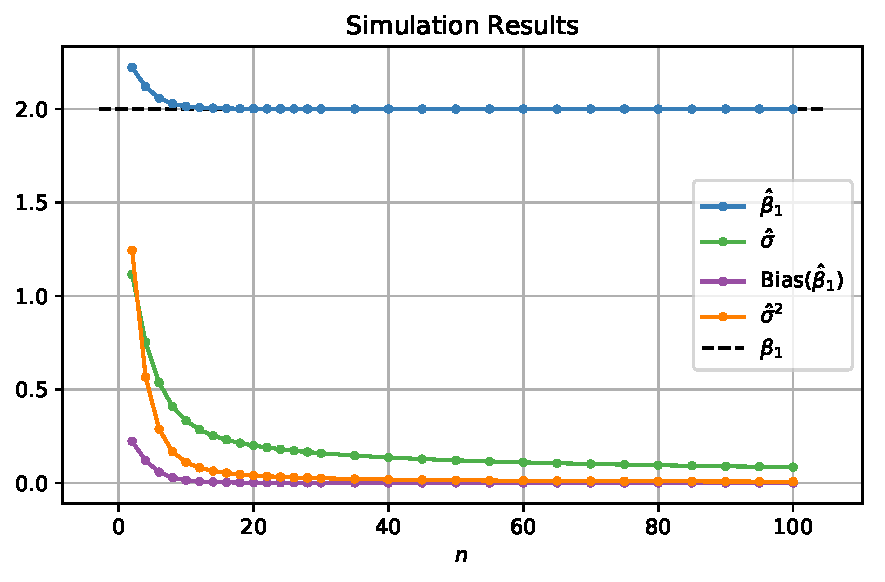
\includegraphics{p1_simulation_results.pdf}
    \caption{Data from Table \ref{tab:p1_simulation_results} along with
      asymptotic slope $\beta_1$.}
    \label{fig:p1_simulation_results}
  \end{figure}

  These data are plotted in Figure \ref{fig:p1_simulation_results}.
\end{description}

{\item Comment on your findings in part (e).  Is the bias in estimating $\beta_1$ surprising?  Why or why not?  How concerned should one be about this bias? }
{\item It is possible to derive exact values for the biases estimated in part (d) by enumerating all possible draws of $x_1, \ldots, x_n$.  Do this calculation for $n=2,4,6,8$.  Report your numerical findings and overlay them on your plot from part (e).   Show how you can do the calculation entirely by hand for $n=2$ (you may use a computer for matrix algebra).  Although it is highly advisable to use a computer for this calculation for $n>2$, simulation results are not sufficient.  Your calculation of the bias must be exactly correct up to the computer's floating point precision.}
\end{enumerate}



\section*{Problem 2: Average slope interpretation of generalized least squares (5 points)}
{\em Consider simple linear regression with a
single covariate and an intercept, such that we are fitting
\[
E(Y_i)=\beta_0 + \beta_1 x_i
\]
with scalar observations $Y_1,\ldots,Y_n$. As we saw on slide 1.18, the OLS estimator of $\beta_1$ can
be written as a weighted average of the pairwise slopes $(Y_i-Y_j)/(x_i-x_j)$.
This is called the ``average slope'' representation.
}
\begin{enumerate}[(a)]
{\em \item Suppose that $\bSigma$, the covariance of $\bY$, is a diagonal matrix with known entries $\sigma_1^2,\ldots,\sigma_n^2$.
Derive the weights for an ``average slope'' representation for the optimal generalized least squares (GLS) estimate of $\beta_1$ (see exercise 8.1 in the Wakefield text if you are not sure of the form of the optimal GLS estimate).  A formal proof is optional, but you should provide a convincing justification for the specific form of your answer.  HINT: One way to approach this problem is to think about what happens when the $\sigma^2_i$ are all rational numbers, i.e., they can be expressed as fractions.}
{\item Now consider what the weights would be in an ``average slope''
representation for the optimal GLS estimate of $\beta_1$, for a general covariance matrix $\bSigma$.  Give some properties of the weights that you would expect to hold.  In answering this question, it might be helpful to think about how the weights would change as you vary individual entries in $\bSigma$.
Also discuss any situations where you would expect the weight for a particular pair of observations to 
be infinite or zero.  Note that you are {\bf not} asked to derive an average slope representation for GLS.}
\end{enumerate} 


\section*{Problem 3: Cross-sectional/longitudinal effects, partitioning the exposure, mean model misspecification (10 points)}
{\em Consider a made-up computer literacy trial similar to the one discussed in lecture (slides 1.35--1.48).  There are $n$ subjects, indexed by $i=1,\ldots,n$, each one of which is observed at
$m$ followup times, indexed by $j=1,\ldots,m$.  Let $Y_{ij}$ be the literacy score of subject $i$ at follow-up time $j$, at which time the subject's age is $x_{ij}$.  Suppose the design is fixed, meaning that the $x_{ij}$ are all
deterministic and known in advance, and assume the true data-generating
mechanism can be written
\begin{equation}
\label{eq1}
Y_{ij}=f(x_{i1})+\beta_L(x_{ij}-x_{i1})+\epsilon_{ij}
\end{equation}
with i.i.d. $\epsilon_{ij}\sim N(0,\sigma^2)$.  The unknown function $f(\cdot)$ 
represents a potentially nonlinear cohort effect and $\beta_L$ is the coefficient for the 
linear longitudinal effect.
Suppose we try to estimate $\beta_L$ using 
the exposure partioning method proposed on slide 1.44
(see, also, Diggle et al. page 16), based on the linear regression estimating equations
with the mean model
\begin{equation}
\label{eq2}
E(Y_{ij})=\beta_0 + \beta_C x_{i1} + \beta_L (x_{ij}-x_{i1}).
\end{equation}}
\begin{enumerate}[(a)]
{\em \item Give a sufficient condition on the data-generating mechanism for $Y_{ij}$ in equation~(\ref{eq1}) to guarantee
unbiased estimation of $\beta_L$ and valid model-based standard errors.}
{\em \item Give a sufficient condition on the choice of follow-up times in the study design to guarantee
unbiased estimation of $\beta_L$, even if the condition in part (a) is violated.  Thinking about
when confounding bias is a problem will be helpful here.}
{\em \item Download the modified made-up literacy data from the course web site (you can find these data with the homework files, not in the general dataset section), and generate
one or more exploratory plots.  Describe how you can graphically see evidence that neither of
the above conditions is satisfied.}
{\em \item Propose an alternative regression model that can still be used to unbiasedly estimate $\beta_L$ and give valid model-based standard errors.  Fit this model to the downloaded data using the $\texttt{lm()}$ function in $\texttt{R}$ and report your findings (point estimate and standard error).
Compare to what you obtain by fitting model~(\ref{eq2}) to the data.}
{\em \item Design and conduct a simulation study to illustrate the following 
\begin{enumerate}
\item Model~(\ref{eq2}) can fail to give unbiased estimates of $\beta_L$ without at least one of the additional conditions from parts (a) and (b).
\item Model~(\ref{eq2}) does give unbiased estimates if either of the additional conditions from parts (a) and (b) is satisfied.
\item The model you propose in part (d) works, regardless.
\end{enumerate}
You will need to consider a few choice of $f(\cdot)$ and study designs $\{x_{ij}\}$
to illustrate points (i) through (iii).  Note that in earlier parts of the problem, you should have 
argued theoretically that each of these points is true; the purpose of the simulation study is to verify
and illustrate your conclusions. }
{\em \item In your simulation study, what do you notice about the standard error estimates from the model in equation~(\ref{eq2}) when the condition from part (b) is satisfied but
the condition from part (a) is not satisfied?  Do sandwich standard errors fix the problem?  }
{\em \item Explain, theoretically, what is going wrong in part (f) of this problem.
This involves some fairly careful thinking about misspecified mean models and what is required
for sandwich estimation to be valid.}
\end{enumerate} 


\end{document}